\documentclass[12pt]{article}
\usepackage{html}
\usepackage{graphicx}
\begin{document}
\author{\htmladdnormallink{The FreeCol
    Team}{http://freecol.sourceforge.net/index.php?section=8}}
\title{FreeCol Documentation\\User Guide v0.1.2}
\maketitle{}
\section{Introduction}
\label{introduction}
Welcome to FreeCol! If you're interested in development of
this program, please see the \htmladdnormallink{FreeCol web
  site}{http://freecol.sourceforge.net}. This is a draft version of
the user's guide. You can find the latest version at the 
\htmladdnormallink{FreeCol
  homepage}{http://freecol.sourceforge.net}.\\

\section{History}
\label{history}
This section gives details about the history of this user guide.
\begin{itemize}
\item v0.1.2: corrections from Bryce Harrington and copyright notice.
\item v0.1.1: Main screen's, Colony panel's and Europe panel's images
  were added.
\item v0.1: Creation of the user guide! The guide contains the
  following sections: �Introduction�, �History�, �Installation� and
  �Interface�.
\end{itemize}

\section{Installation}
\label{installation}
To compile FreeCol you'll need Java and the Ant program. Ant can be
found at \htmladdnormallink{Ant homepage}{http://ant.apache.org/}.\\

When these are installed, go to the root directory of
FreeCol and type \verb$ant$ to build a JAR file containing the
game. The game is started using the command \verb$java -jar FreeCol.jar$.
If something goes wrong, send a bug report at the
\htmladdnormallink{SourceForge page of
  FreeCol}{http://sourceforge.net/projects/freecol}.

\section{Interface}
\label{interface}
This section will provide information about the keyboard shortcuts and
the different actions that can be used in the game.

\subsection{The main screen}
\label{main_screen}
The figure \ref{main_screen_fig} represents the main screen.
\begin{figure}
  \begin{center}
    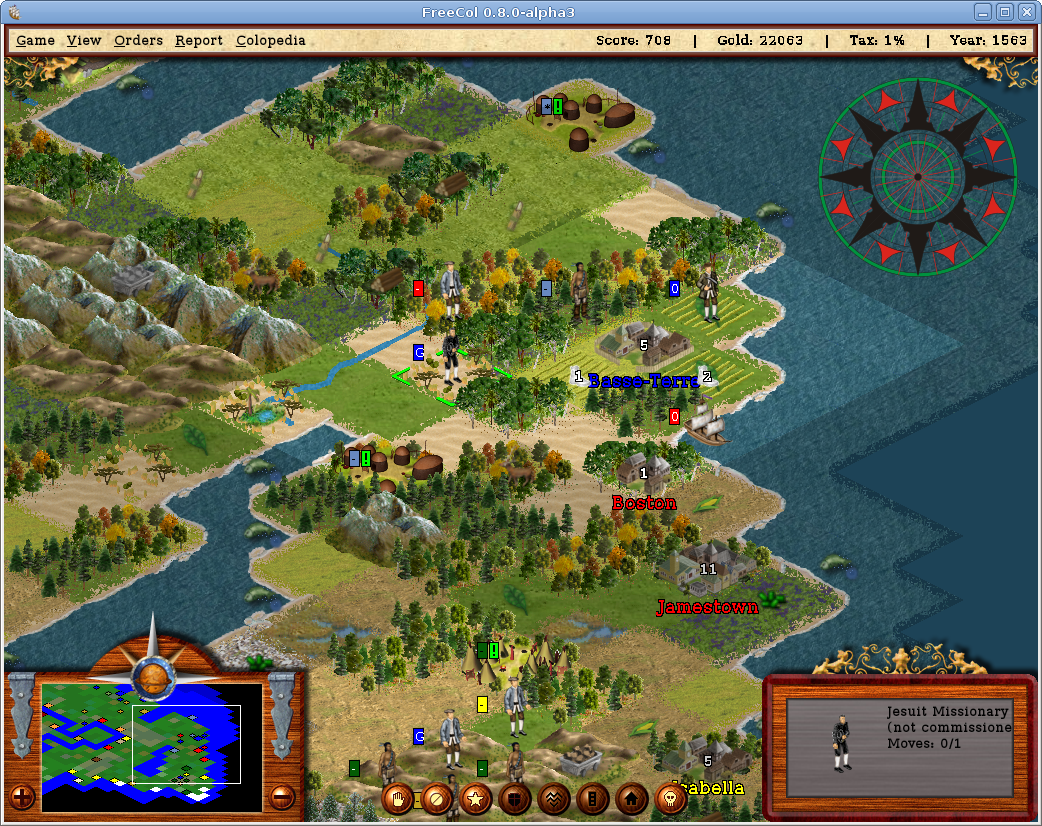
\includegraphics[scale=0.975]{images/main_screen.png}
    \caption{The main screen.\label{main_screen_fig}}
  \end{center}
\end{figure}

The units, colonies, and so forth can be seen on the main screen. You
can move the currently selected unit using the numeric keypad. You can
change the currently selected unit by clicking on any other unit. If
you right click on a tile, you can see the different units that are on
this tile.\\

The following shortcuts are also available:
\begin{itemize}
\item\verb$w$: wait.
\item\verb$space$: skip for this turn.
\item\verb$f$: fortify.
\item\verb$s$: sentry.
\item\verb$p$: plow the current tile.
\item\verb$r$: build a road on the current tile.
\item\verb$b$: build a colony.
%% disband
\item\verb$c$: center on the currently selected unit.
\item\verb$enter$: end the turn.
\item\verb$ctrl-e$: show the Europe panel.
\item\verb$ctrl-t$: show the chat panel.
\item\verb$plus$ or \verb$equals$: zoom in.
\item\verb$minus$ or \verb$underscore$: zoom out.
\item\verb$ctrl-n$: new game.
\item\verb$ctrl-o$: open a game.
\item\verb$ctrl-s$: save a game.
\item\verb$ctrl-r$: reconnect.
\item\verb$ctrl-q$: quit the game.
\item\verb$ctrl-m$: show/hide the map controls.
\item\verb$ctrl-d$: display tile names.
\item\verb$ctrl-g$: display grid.
\end{itemize}

\subsection{The Europe panel}
\label{europe_panel}
The figure \ref{europe_panel_fig} represents the Europe panel.
\begin{figure}
  \begin{center}
    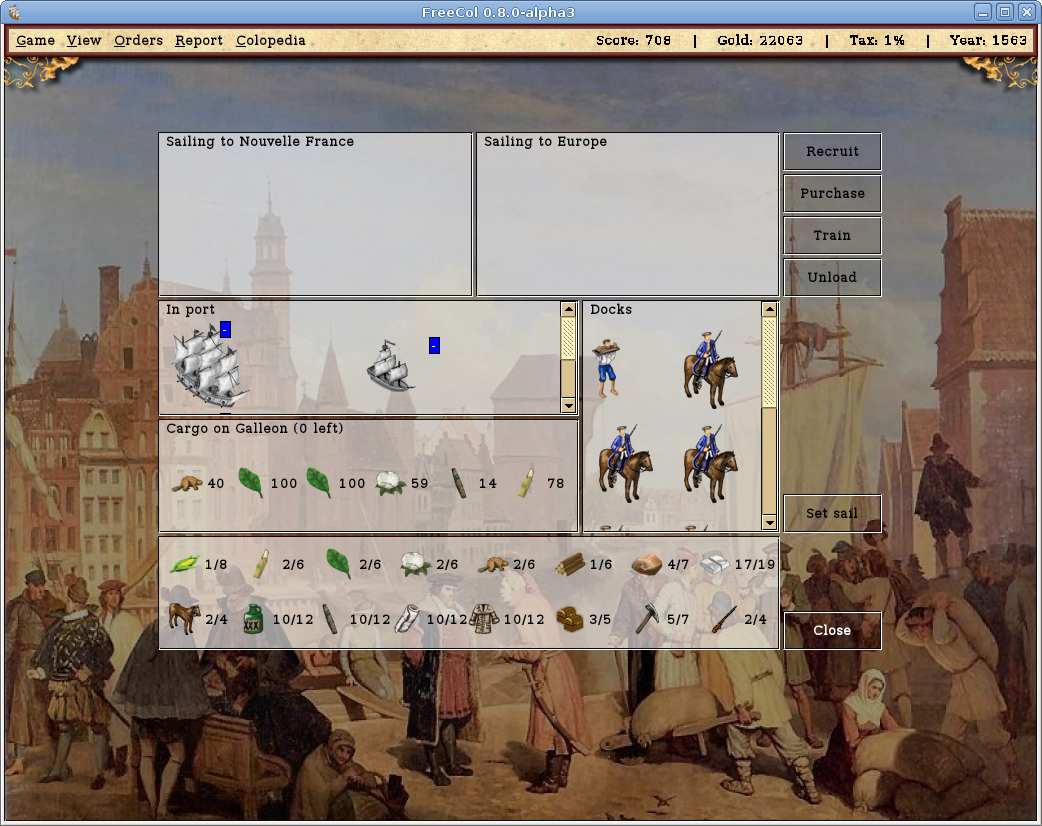
\includegraphics[scale=0.975]{images/europe_panel.png}
    \caption{The Europe Panel.\label{europe_panel_fig}}
  \end{center}
\end{figure}

In this panel, you can control the ships embarked for America or Europe,
and the ships currently stationed in Europe. You can also buy goods,
recruit, purchase and train units. Units recruited, purchased or trained
are in the �Docks� area in the Europe panel.\\

If a ship has set sail for Europe or America, you can change its
direction.\\

Ships that are docked at the European port can also do the following:
\begin{itemize}
\item Embark/Disembark units: drag and drop between the �Docks�
  and �Cargo� sections of the Europe panel.
\item Sell/Buy goods: drag and drop between the �Cargo� part of
  the Europe panel and the part of the Europe panel where all the
  goods are listed. If you want to sell/buy only a part of a type of
  goods, use the shift key while dropping it.
\item Arm/Mount/Equip with tools/Dress as missionaries a unit: 
  right click on the unit.
\item Move your ship to the �Going to America� section of the Europe
  panel.
\end{itemize}

\subsection{The Colony panel}
\label{colony_panel}
The figure \ref{colony_panel_fig} represents the Colony panel.
\begin{figure}
  \begin{center}
    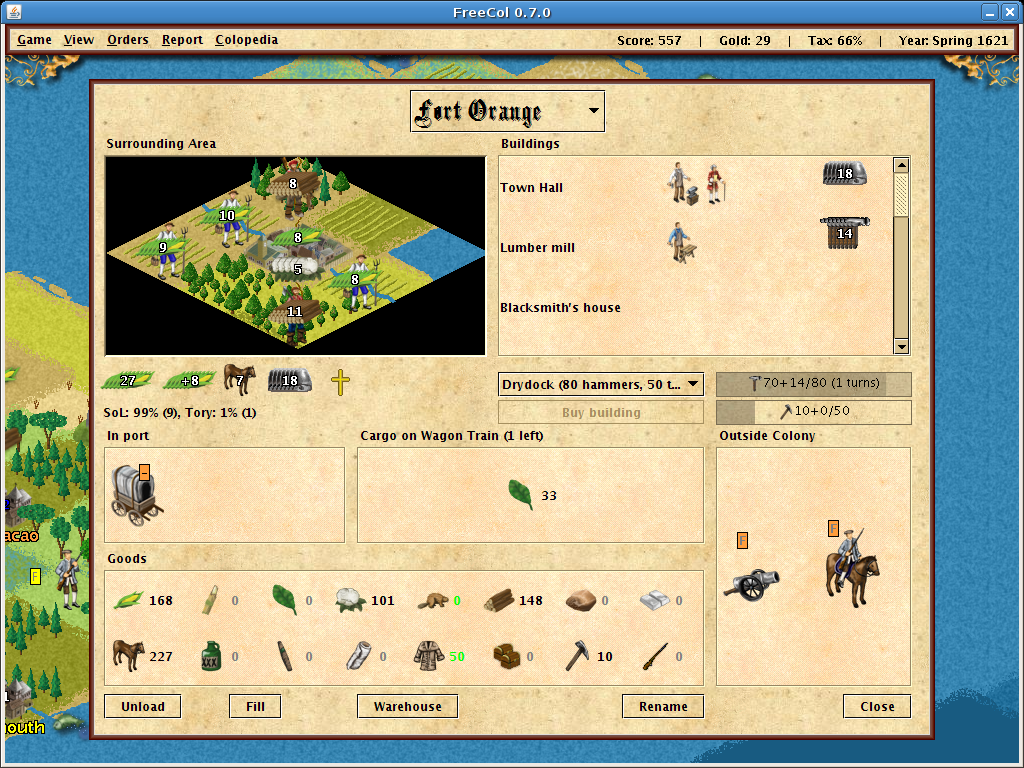
\includegraphics[scale=0.975]{images/colony_panel.png}
    \caption{The Colony Panel.\label{colony_panel_fig}}
  \end{center}
\end{figure}

To view a colony's panel, left click on it from the main
screen. From this panel, colonist's cultivation, production, and other
tasks can be assigned:
\begin{itemize}
\item Cultivation: Drop the unit onto the appropriate plot of land in
  the colony. You can change what a colonist cultivate by right
  clicking on it.
\item Production: Drop the unit onto the relevant �Buildings�.
\item Depart colony: Drop the unit onto the colony's gate.
\item Embark on a ship: If there is a ship in port, you can embark
  your colonist on it by dropping it onto the �Cargo� section of the
  colony panel.
\end{itemize}

You can also load cargo into a ship's hold by dropping the goods onto
the ship or the specific hold within the ship. Use the shift key while
dropping it if you want to load only a portion of the goods.

\section{Copyright Notice}
Copyright � 2004 \htmladdnormallink{The FreeCol
  Team}{http://freecol.sourceforge.net/index.php?section=8}.\\

This manual is free software; you may redistribute it and/or modify it
under the terms of the GNU General Public License as published by the
Free Software Foundation; either version 2, or (at your option) any
later version.\\

This is distributed in the hope that it will be useful, but without
any warranty; without even the implied warranty of merchantability or
fitness for a particular purpose. See the GNU General Public License
for more details.\\

A copy of the GNU General Public License is available on the World
Wide Web at \htmladdnormallink{the GNU General Public
  Licence}{http://www.gnu.org/copyleft/gpl.html}. You can also obtain
it by writing to the Free Software Foundation, Inc., 59 Temple Place -
Suite 330, Boston, MA 02111-1307, USA.

\end{document}
